\documentclass[aip,adv,reprint,onecolumn,amsmath,amssymb]{revtex4-2}
\usepackage{cmap}
\usepackage[T1]{fontenc}
\usepackage{mathptmx,bm,amsthm,graphicx,booktabs,hyperref}
\hypersetup{hidelinks,pdftitle={Coherent Saddle Encoding and Displacement Recovery: Residual-State Criteria and Timing Limits},pdfauthor={Jason Duran Dutton}}
\graphicspath{{figures/}}
\setlength{\emergencystretch}{2em}
\newcommand{\R}{\mathbb R}
\newcommand{\C}{\mathbb C}
\newcommand{\Id}{\mathbb 1}
\newcommand{\ii}{\mathrm i}
\newcommand{\dd}{\mathrm d}
\newcommand{\Tr}{\operatorname{Tr}}
\newcommand{\ket}[1]{\lvert #1\rangle}
\newcommand{\bra}[1]{\langle #1\rvert}
\newcommand{\Ph}{\boldsymbol\phi}
\newcommand{\Jm}{\operatorname{diag}(1,-1)}
\newtheorem{theorem}{Theorem}[section]
\newtheorem{proposition}[theorem]{Proposition}
\newtheorem{corollary}[theorem]{Corollary}
\newtheorem{definition}[theorem]{Definition}
\begin{document}
\title{Coherent Saddle Encoding and Displacement Recovery: Residual-State Criteria and Timing Limits}
\author{Jason Duran Dutton}
\thanks{ORCID: \href{https://orcid.org/0009-0004-8655-9901}{0009-0004-8655-9901}}
\affiliation{Independent Researcher, Castlewood, Virginia 24224, USA}
\date{November 25, 2026}
\begin{abstract}
Recovery of quantum information requires preservation of unknown amplitudes and reference entanglement, rather than restoration of classical coordinates alone. We construct a coherent saddle encoding with a conditional two-oscillator realization and characterize its recovery under label-preserving random-unitary noise. A necessary and sufficient criterion requires the decoded auxiliary state vectors, including their relative phases, to coincide across logical labels for almost every disturbance. Their mean squared separation equals an entanglement-fidelity deficit and gives a sufficient channel-distance estimate. At a common half-period, the complete oscillator encoder contains a saddle displacement, its companion displacement, parity and a calculable logical phase. Its coherent inverse followed by auxiliary trace exactly recovers every logical state under arbitrary probability mixtures of common auxiliary translations. At general evolution times with a matched inverse decoder, Gaussian translations produce an explicit dephasing kernel and a quadratic timing-error coefficient. Exact finite-register checks, direct oscillator evolution, cutoff refinement and reference-entanglement tests verify the stated realizations. Differential shifts, discarded companion information, phase gradients and erasure provide explicit limits. Matched flat and conventional controls identify established subsystem protection rather than an intrinsic benefit of saddle curvature. A finite path-and-transverse-mode optical mapping is proposed with its approximations stated. Appendices retain the constrained scalar-field, localization, coherent-history and conditional geometric calculations, without treating them as a microscopic derivation of the recovery channel.
\end{abstract}
\maketitle

\section{Introduction}
Returning a classical point to a surface does not establish recovery of encoded quantum information. A procedure can restore coordinates while changing relative phases or leaving the logical label in an unobserved auxiliary system. A recovery claim must instead specify a state space, encoding, noise and decoding, and test their composition on arbitrary inputs, including inputs entangled with an untouched reference. The error-correction conditions and entanglement fidelity provide established criteria.\cite{knill,nielsen}

We study a controlled translation encoding whose design height is the saddle $h(x,y)=\alpha x^2-\beta y^2$. The full dynamical construction uses two forced harmonic oscillators. Their difference coordinate has the chosen saddle displacement, but their sum also acquires a label-dependent displacement. Both coordinates, their parity and the logical phase are retained in the encoder and decoder. Design labels identify control settings; they are not unknown classical coordinates measured during recovery.

The central result is a residual-state criterion for a specified class of controlled encodings and label-preserving random-unitary errors. It gives an identity-channel condition, an exact entanglement-fidelity deficit, and a sufficient diamond-norm estimate. In the oscillator realization it yields exact common-translation recovery at shared turning times and a Gaussian dephasing law away from those times. The timing law assumes decoding by the coherent inverse of the actual encoder; independent encoder and decoder timing errors are a different problem addressed by the general residual-state test.

The protection is an instance of established subsystem error correction.\cite{kribs} A controller implementing the same operations, or a matched flat construction with label-independent shifts, has the same common-translation protection. The contribution is the explicit coherent realization, the quantitative recovery criteria and the timing and error boundaries, rather than a new general error-correction principle or a demonstrated performance advantage.

The main text develops the quantum construction independently of a classical-field interpretation. Appendices give the complementary mathematics: a constrained conjugate representation of one complex scalar, a positive internal-response extension, a localization benchmark, coherent histories, limits of positive trajectory reconstruction, and conditional geometric and prescribed-background examples. These have separate assumptions. No quantization of that scalar system into the optical register, or common microscopic coupling across the examples, is derived. This separation lets the quantum result be evaluated without assuming those additional physical connections.

\section{Registers, operations and recovery criteria}
\label{sec:registers}
\subsection{Logical modes and prepared auxiliary coordinates}
Let $\mathcal H_L=\C^d$ have orthonormal logical basis $\{\ket b\}_{b=0}^{d-1}$. A known design point $r_b=(x_b,y_b)$ is assigned to each label in a bounded design set. The input $\rho$ is arbitrary and unknown; the controls depend on $b$ through the known design, not on the amplitudes of $\rho$. The auxiliary space is initially an arbitrary Hilbert space $\mathcal H_A$ with a fixed normalized packet $g$. The oscillator realization specializes to $\mathcal H_A=L^2(\R^2,\dd q_1\dd q_2)$ with $[Q_a,P_c]=\ii\hbar\delta_{ac}$. Its canonical translations act as
\begin{equation}
 T(\bm d)=e^{-\ii\bm d\cdot\bm P/\hbar},\qquad
 [T(\bm d)g](\bm q)=g(\bm q-\bm d).
 \label{eq:translation-definition}
\end{equation}
The two dynamical coordinates are also denoted $S,W$ in some figures and numerical scripts: $Q_S=Q_1$, $Q_W=Q_2$. The reference register is separate and untouched.

For assigned displacement vectors $\bm h_b$, the direct geometric shear is
\begin{equation}
 U_h=\sum_b\ket b\bra b\otimes T(\bm h_b),\qquad
 V_h\ket\psi=U_h(\ket\psi\otimes\ket g).
 \label{eq:direct-shear}
\end{equation}
Translation unitarity makes $U_h$ unitary and $V_h$ isometric. The oscillator encoder below additionally contains parity and a known logical phase. Its quantum register and canonical commutation relations are explicit assumptions, not consequences of a classical conjugate-pair notation.

\begin{figure}[tb]
\centering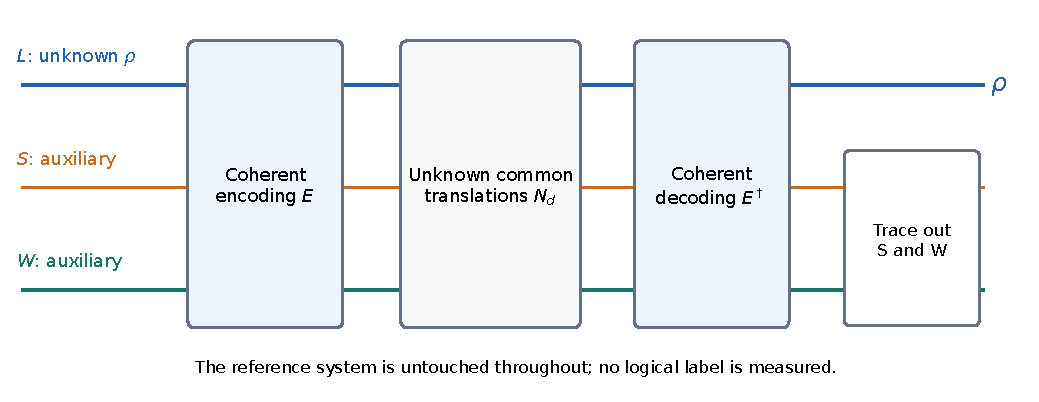
\includegraphics[width=.98\linewidth]{figure_1_registers.pdf}
\caption{Coherent register operations. The unknown logical state is encoded with two prepared auxiliaries, disturbed by common auxiliary translations, and decoded coherently. Both auxiliaries are traced only after decoding. An external reference is untouched. $L$ denotes the logical register, and $S,W$ denote auxiliary coordinates 1,2. The diagram is a channel schematic, not a fabricated device.}
\label{fig:registers}
\end{figure}

\subsection{Retraction and controlled quantum operations}
For a smooth graph $z=h(x,y)$ in Euclidean design coordinates, the map $(x,y,z)\mapsto(x,y,h(x,y))$ is a vertical retraction. It need not be a nearest-point projection. A smooth embedded Riemannian submanifold admits a nearest-point map locally in an appropriate tubular neighborhood; global uniqueness requires more.\cite{docarmo} Lorentzian spacetime does not supply a positive distance to minimize in the same way.

A point retraction also need not preserve an operator eigenvalue. On the circle, $A=-\partial_x^2$ has eigenfunction $e^{\ii nx}$ with eigenvalue $n^2$. Pullback by the constant retraction $\pi(x)=0$ gives the constant function one, whose eigenvalue is zero for $n\ne0$. A spectral projection obtained from the self-adjoint functional calculus commutes with its operator;\cite{reed} an arbitrary geometric retraction does not inherit that property.

These distinctions motivate an operational construction. Let $\mathcal H_L=\C^d$ have orthonormal logical modes $\ket b$, and let $\mathcal H_A$ be an auxiliary Hilbert space prepared in a normalized packet $g$. Choose known unitaries $E_b$ and define
\begin{equation}
 E=\sum_{b=0}^{d-1}\ket b\bra b\otimes E_b,\quad
 V\ket\psi=E(\ket\psi\otimes\ket g),\quad
 \mathcal D_E(\tau)=\Tr_A(E^\dagger\tau E).
 \label{eq:encoder}
\end{equation}
Encoding by $V$ and decoding by $\mathcal D_E$ are completely positive and trace preserving on their appropriate spaces. The logical amplitudes are unknown; the branch controls are specified independently of them. For $d=2$, the logical labels denote two orthogonal calibrated modes. Identifying them with classical frequency sectors would require an additional mode assignment beyond \eqref{eq:embedding}.

Let $\omega$ label a random disturbance with probability measure $\mu$, and suppose the noise preserves the logical labels while applying auxiliary unitaries $W_{b,\omega}$:
\begin{equation}
 N_\omega=\sum_b\ket b\bra b\otimes W_{b,\omega},\qquad
 \mathcal N(\tau)=\int N_\omega\tau N_\omega^\dagger\,\mu(\dd\omega).
 \label{eq:controlled-noise}
\end{equation}
Assume the stated families are measurable so these trace-class integrals exist. Label mixing and erasure are different channels considered separately below.


To fix the recovery metric, let $\Lambda(\rho)=\mathcal D_E\mathcal N(V\rho V^\dagger)$. Exact recovery means $\Lambda=\operatorname{id}_L$ on every logical operator, including off-diagonal matrix units. Define
\begin{equation}
 \ket{\Omega_d}=\frac1{\sqrt d}\sum_b\ket b_{\mathrm{ref}}\ket b_L,
 \qquad F_e(\Lambda)=\bra{\Omega_d}(\operatorname{id}_{\mathrm{ref}}\otimes\Lambda)
 (\ket{\Omega_d}\bra{\Omega_d})\ket{\Omega_d}.
 \label{eq:reference-fidelity}
\end{equation}
This is an unconditional overlap; projection failures and erasures are not removed by postselection.

\subsection{Residual-state theorem and quantitative approximation}
\begin{theorem}[Residual-state criterion and fidelity identity]
\label{thm:residual}
Put $\chi_b(\omega)=E_b^\dagger W_{b,\omega}E_bg$. The recovered logical channel is
\begin{equation}
 [\Lambda(\rho)]_{bc}=\rho_{bc}\,\Gamma_{bc},\qquad
 \Gamma_{bc}=\int\langle\chi_c(\omega),\chi_b(\omega)\rangle\,\mu(\dd\omega).
 \label{eq:gram-channel}
\end{equation}
It is the identity on every input, including inputs entangled with an untouched reference, if and only if all $\chi_b(\omega)$ are equal for $\mu$-almost every $\omega$. For the maximally entangled $d$-level input, its entanglement fidelity obeys
\begin{align}
 F_e(\Lambda)&=\frac1{d^2}\sum_{b,c}\Gamma_{bc}
 =\int\left\|\frac1d\sum_b\chi_b(\omega)\right\|^2\mu(\dd\omega),\label{eq:Fe}\\
 1-F_e(\Lambda)&=\frac1{2d^2}\sum_{b,c}\int
 \|\chi_b(\omega)-\chi_c(\omega)\|^2\,\mu(\dd\omega).
 \label{eq:dispersion}
\end{align}
\end{theorem}
\begin{proof}
Apply the sequence to a matrix unit $\ket b\bra c$. After decoding, the auxiliary operator is $\ket{\chi_b}\bra{\chi_c}$, whose trace gives \eqref{eq:gram-channel}. Since every $\chi_b$ is normalized, $\Gamma_{bb}=1$. Exact identity requires and is implied by $\Gamma_{bc}=1$ for every pair. The identity
\begin{equation}
 \int\|\chi_b-\chi_c\|^2\dd\mu=2-2\operatorname{Re}\Gamma_{bc}
 \label{eq:pair-distance}
\end{equation}
then implies equality almost everywhere; there are finitely many pairs, so a common null set suffices. Conversely equality makes every Gram entry one. Tensoring the matrix-unit calculation with arbitrary reference operators preserves the result. Expanding the maximally entangled state gives the first expression in \eqref{eq:Fe}. Expanding the squared mean and the pairwise squared distances proves \eqref{eq:dispersion}.
\end{proof}

Residual packets equal only up to label-dependent phases generally give a logical phase gate, not the identity. Known phases can be compensated; unknown disturbance-dependent relative phases cannot be omitted. Equations \eqref{eq:gram-channel}--\eqref{eq:dispersion} are a direct expression of the environmental-information principle underlying quantum error correction.\cite{knill,kribs,nielsen} They are used here as a concrete criterion for the proposed construction, not a replacement for the general theory.

\begin{corollary}[A dimension-independent sufficient estimate]
If for a fixed label 0,
\begin{equation}
 \max_b\int\|\chi_b(\omega)-\chi_0(\omega)\|^2\,\dd\mu\le\varepsilon^2,
 \label{eq:approx-condition}
\end{equation}
then $1-F_e\le\varepsilon^2$ and $\|\Lambda-\operatorname{id}\|_\diamond\le\min(2,2\varepsilon)$.
\end{corollary}
\begin{proof}
Regard $\omega\mapsto\chi_b(\omega)$ as a vector $X_b$ in $L^2(\mu;\mathcal H_A)$. The map $\ket b\mapsto\ket b\otimes X_b$ is an isometric dilation of \eqref{eq:gram-channel}. Compare it with $\ket b\mapsto\ket b\otimes X_0$, a dilation of the identity. Orthogonality of the logical basis makes their operator-norm difference at most $\varepsilon$. The elementary trace-distance bound between the output pure states is at most $2\varepsilon$, also with a reference; contraction under partial trace gives the diamond bound. Finally, \eqref{eq:dispersion} is the mean variance of the $X_b$, and the mean minimizes squared distance to a common vector. It is therefore no larger than $d^{-1}\sum_b\|X_b-X_0\|^2$.
\end{proof}
This estimate is consistent with the established continuity theory of channel dilations.\cite{ksw} It states a sufficient bound for this particular diagonal-noise setting.


Equality in Theorem~\ref{thm:residual} concerns normalized complex vectors, not only equal auxiliary density matrices: label-dependent scalar phases can still rotate the logical state. A common disturbance-dependent phase is harmless. For a fixed mixed auxiliary preparation, one can purify it into an additional untouched auxiliary factor and apply the same criterion. The operator factorization used below also proves exact common-translation recovery directly for every auxiliary density operator.
\section{Dynamical realization of the coherent saddle encoder}\label{sec:dynamics}
\subsection{Prescribed geometry and a bounded Hamiltonian}
Take two auxiliary coordinates with $[Q_a,P_c]=\ii\hbar\delta_{ac}$, $a,c\in\{1,2\}$, on $\mathcal H_A=L^2(\R^2)$. At each logical design label $b$, prescribe regular geometric values $\kappa_b>0$, $\tau_b$ and forces $J_{1b}=\mu_1\kappa_b^2$, $J_{2b}=\mu_2\tau_b^2$, with positive couplings. For common mass $M$ and stiffness $k$, the restricted classical Lagrangian and its canonical quantum realization are
\begin{align}
 L_b&=\sum_{a=1}^2\left(\frac M2\dot q_a^2-\frac k2q_a^2-J_{ab}q_a\right),\\
 H_b&=\sum_{a=1}^2\left(\frac{P_a^2}{2M}+\frac k2Q_a^2+J_{ab}Q_a\right),\qquad\omega_0=\sqrt{k/M}.
 \label{eq:oscillators}
\end{align}
The auxiliary oscillator coordinates are not the two entries of \eqref{eq:embedding}. They are additional controlled degrees of freedom in a conditional realization. Prescribed forces and canonical quantization are assumptions. In particular, two independently prescribed geometric forces are not derived from the single density-source direction $\bm h\rho$ in \eqref{eq:coupled}.


An illustrative classical coupling before this restriction is
\begin{equation}
 U_{\mathrm{int}}=\gamma_1(I_0)\kappa^2q_1+\gamma_2(I_0)\tau^2q_2.
 \label{eq:prescribed-source-coupling}
\end{equation}
Selecting constant positive $\gamma_1,\gamma_2$ removes the derivative drive of a possible spectator $I_0$ from this term. With $\gamma_1=\mu_1$ and $\gamma_2=\mu_2$, the prescribed forces are $J_{1b}=\mu_1\kappa_b^2$ and $J_{2b}=\mu_2\tau_b^2$. This is a conditional oscillator sector, not a reduction derived from the reciprocal mediator equations in Appendix~\ref{app:internal}. Other uncoupled spectators may remain in fixed product states.

For a finite set of labels the force values are bounded, and square completion gives a uniform lower bound $H_b\ge-(J_{1b}^2+J_{2b}^2)/(2k)$. The displaced harmonic-oscillator Hamiltonians are essentially self-adjoint on the Schwartz core. The lower bound concerns this prescribed-geometry problem; no unconstrained higher-derivative worldline Hamiltonian is being quantized.

Define $T(\bm d)=\exp[-\ii\bm d\cdot\bm P/\hbar]$ and $(\Pi_Ag)(\bm q)=g(-\bm q)$. For one oscillator, square completion and free half-period evolution give
\begin{equation}
 e^{-\ii t_*H_J/\hbar}=e^{\ii\pi J^2/(2k\hbar\omega_0)-\ii\pi/2}\,T(-2J/k)\Pi,
 \qquad t_*=\pi/\omega_0.
 \label{eq:half-period}
\end{equation}
For completeness, write $q_*=-J/k$ and $H_J=T(q_*)H_0T(q_*)^\dagger-J^2/(2k)$. Since $e^{-\ii\pi H_0/(\hbar\omega_0)}=e^{-\ii\pi/2}\Pi$ and $\Pi T(a)=T(-a)\Pi$, \eqref{eq:half-period} follows without an impulsive approximation.

The full controlled encoder has branches
\begin{equation}
 E_b=e^{\ii\varphi_b}T(\bm h_b)\Pi_A,\quad
 \bm h_b=-\frac2k(J_{1b},J_{2b}),\quad
 \varphi_b=\frac{\pi(J_{1b}^2+J_{2b}^2)}{2k\hbar\omega_0}-\pi.
 \label{eq:complete-encoder}
\end{equation}
Both parity and the branch phase are part of the coherent operation. Since $E_b^2=e^{2\ii\varphi_b}\Id$, a second forward half-period followed by the known logical phase $\operatorname{diag}(e^{-2\ii\varphi_b})$ implements $E^\dagger$. The inverse need not be interpreted as backward physical time.


Explicitly, if $D=\sum_b e^{-2\ii\varphi_b}\ket b\bra b$, then
\begin{equation}
 E^\dagger=(D\otimes\Id_A)E,\qquad E=\sum_b\ket b\bra b\otimes E_b.
 \label{eq:forward-decoder}
\end{equation}
Both controls are known functions of the prescribed forces. A forward half-period and this phase operation synthesize the inverse at the half-period; control accuracy remains an implementation requirement.
\subsection{Difference and companion coordinates}
The canonical rotation
\begin{equation}
 Z=\frac{Q_2-Q_1}{\sqrt2},\qquad B=\frac{Q_2+Q_1}{\sqrt2}
 \label{eq:ZB}
\end{equation}
has the corresponding momentum rotation and preserves the equal-parameter free quadratic form. For bounded design labels $(x_b,y_b)$, choose
\begin{equation}
 J_{1b}=J_0+\frac{k\alpha x_b^2}{\sqrt2},\qquad
 J_{2b}=J_0+\frac{k\beta y_b^2}{\sqrt2},\qquad J_0,\alpha,\beta>0.
 \label{eq:forces}
\end{equation}
The resulting displacements are
\begin{equation}
 h_{Zb}=\alpha x_b^2-\beta y_b^2,\qquad
 h_{Bb}=-\frac{2\sqrt2J_0}k-\alpha x_b^2-\beta y_b^2.
 \label{eq:saddle}
\end{equation}
Thus the signed saddle comes from a difference of two nonnegative force profiles. Its sum coordinate remains present and can carry branch information. Equation \eqref{eq:forces} is a design prescription, not a consequence that curvature and torsion must satisfy. Positive prescribed curvatures are kinematically admissible as described in Appendix~\ref{app:geometry}.


The momentum rotation is $P_Z=(P_2-P_1)/\sqrt2$, $P_B=(P_2+P_1)/\sqrt2$; it preserves the canonical commutators. Before inserting the quadratic design,
\begin{equation}
 h_{Zb}=\frac{\sqrt2}{k}(J_{1b}-J_{2b}),\qquad
 h_{Bb}=-\frac{\sqrt2}{k}(J_{1b}+J_{2b}).
 \label{eq:force-to-coordinate}
\end{equation}
On $|x_b|\le L_x$, $|y_b|\le L_y$, square completion gives the explicit uniform bound
\begin{equation}
 H\ge-\frac{(J_0+k\alpha L_x^2/\sqrt2)^2+(J_0+k\beta L_y^2/\sqrt2)^2}{2k}\Id.
 \label{eq:bounded-design}
\end{equation}
This bound is for bounded prescribed controls. It is not a nonlinear stability theorem for dynamic geometry, and the unrestricted-plane prescription does not give this uniform bound.

\begin{figure}[tb]
\centering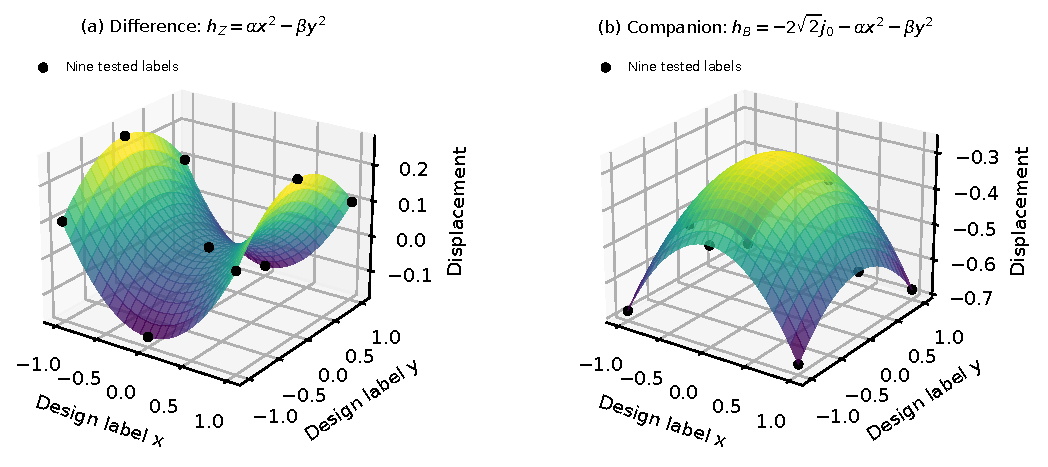
\includegraphics[width=.98\linewidth]{figure_2_surfaces.pdf}
\caption{Both encoded displacements for $k=1$, $J_0=0.1$, $\alpha=0.25$, $\beta=0.15$. The difference coordinate gives the chosen saddle, while the sum gives its companion. Black points identify the nine tested design labels; surfaces are the analytic prescription. These are dimensionless control labels and displacements. The two positive force profiles are prescribed, rather than selected by the curvature--torsion coupling.}
\label{fig:surfaces}
\end{figure}
\section{Exact recovery under common auxiliary translations}\label{sec:recovery}
Let $\mu$ be any probability measure on $\R^2$ and
\begin{equation}
 \mathcal N_\mu(\tau)=\int (\Id_L\otimes T(\bm d))\tau(\Id_L\otimes T(\bm d)^\dagger)\,\mu(\dd\bm d).
 \label{eq:translation-noise}
\end{equation}
At $t_*$, translations commute and parity reverses their sign, so
\begin{equation}
 E_b^\dagger T(\bm d)E_b=T(-\bm d),\qquad
 E^\dagger(\Id_L\otimes T(\bm d))E=\Id_L\otimes T(-\bm d).
 \label{eq:factorization}
\end{equation}
The residual states are identical for all labels. The residual-state criterion in Theorem~\ref{thm:residual} immediately gives exact recovery for every logical state and reference extension. No small-shift approximation, known realization of $\bm d$, or Gaussian hypothesis is required.


\begin{corollary}[Exact common-translation logical channel]
For the complete half-period encoder in \eqref{eq:complete-encoder}, every prepared normalized auxiliary packet and every probability measure in \eqref{eq:translation-noise} satisfy
\begin{equation}
 \mathcal D_E\circ\mathcal N_\mu\circ\mathcal E_E=\operatorname{id}_L,
 \qquad\mathcal E_E(\rho)=V\rho V^\dagger.
 \label{eq:exact-channel}
\end{equation}
The equality remains valid after tensoring with any untouched reference.
\end{corollary}
\begin{proof}
For a fixed shift and any matrix unit $\ket b\bra c$, \eqref{eq:factorization} leaves
\begin{equation}
 \ket b\bra c\otimes T(-\bm d)\ket g\bra gT(-\bm d)^\dagger.
 \label{eq:recovered-matrix-unit}
\end{equation}
The auxiliary trace is one. Integration against a probability measure leaves every matrix unit unchanged, and reference operators are untouched. The same factorization applies to a mixed auxiliary density operator.
\end{proof}
No syndrome measurement is required for this realization: the residual auxiliary state may depend on the disturbance but not on the logical label. Measuring the logical label before coherent decoding instead dephases the input. For a qubit maximally entangled with a reference, that measurement gives $F_e=1/2$, although its basis-state populations are correct.

For a finite mixture with Kraus operators $A_j=\sqrt{p_j}(\Id\otimes T(\bm d_j))$, the encoding isometry explicitly satisfies
\begin{equation}
 V^\dagger A_j^\dagger A_\ell V=\sqrt{p_jp_\ell}\langle g,T(\bm d_j-\bm d_\ell)g\rangle\Id_L.
 \label{eq:KL}
\end{equation}
This is the Knill--Laflamme condition.\cite{knill} The auxiliary residuals need not be orthogonal. In decoded coordinates the logical factor is noiseless, placing the construction within ordinary subsystem protection.\cite{kribs} A flat, label-independent displacement and a conventional controller implementing the same operations have the same common-translation protection.


\subsection{Matched conventional and flat controls}
In decoded coordinates the logical subsystem is noiseless. A conventional controller implementing the same $E,E^\dagger$ gives the same channel. Saddle curvature is therefore unnecessary for the stated common-translation protection; the dynamical construction explains how the chosen displacement, phase and companion can be retained coherently, rather than improving the general error-correction criterion.
\section{Timing errors and the boundary of exact recovery}
\subsection{Exact evolution at a general time}
The time-dependent experiment uses $E(t)$ for encoding and its exact coherent inverse $E(t)^\dagger$ for decoding, with the disturbance between them. Thus the deviation from $t_*$ is a matched change of the encoding operation. If an experimental decoder instead repeats a forward evolution with a nominal half-period phase compensation, it realizes the inverse only at the stated half-period; that different off-time experiment does not automatically obey the following law. For a mismatched decoder $F$, the general theorem applies after replacing the residual definition by $\chi_b=F_b^\dagger W_{b,\omega}E_bg$ and using the resulting Gram kernel. Independent timing and control errors must be specified there.

Allow each auxiliary mode to have positive $M_a,k_a$ and $\omega_a=\sqrt{k_a/M_a}$, fixed across logical labels. The controlled branch is $E_b(t)=e^{-\ii tH_b/\hbar}$. Heisenberg evolution on the oscillator core gives
\begin{equation}
 E_b(t)^\dagger P_aE_b(t)=P_a\cos\omega_at-M_a\omega_aQ_a\sin\omega_at
 -\frac{J_{ab}}{\omega_a}\sin\omega_at.
 \label{eq:Heisenberg}
\end{equation}
Exponentiating the corresponding Weyl operator extends the identity to all normalized packets. Hence
\begin{equation}
 E_b(t)^\dagger T(\bm d)E_b(t)=e^{\ii\bm d\cdot\bm f_b(t)}W_t(\bm d),\qquad
 f_{ab}(t)=\frac{J_{ab}}{\hbar\omega_a}\sin\omega_at,
 \label{eq:time-commutation}
\end{equation}
where $W_t(\bm d)$ is a common auxiliary unitary independent of $b$. Thus a disturbance that is common before decoding can leave a branch-dependent phase at an imperfect evolution time.

\begin{theorem}[Gaussian recovery criterion at arbitrary time]
For common translation noise with Gaussian mean $\overline{\bm d}$ and covariance $C_d\ge0$, the effective logical channel at time $t$ has
\begin{equation}
 \Gamma_{bc}(t)=\exp\left[\ii\overline{\bm d}\cdot\bm\ell_{bc}(t)-\tfrac12\bm\ell_{bc}(t)^TC_d\bm\ell_{bc}(t)\right],
 \quad \bm\ell_{bc}(t)=\bm f_b(t)-\bm f_c(t).
 \label{eq:timing-kernel}
\end{equation}
After compensation of the known mean phase, recovery is the identity if and only if $C_d^{1/2}\bm\ell_{bc}(t)=0$ for every pair. In particular, for positive-definite covariance this requires
\begin{equation}
 (J_{ab}-J_{ac})\sin\omega_at=0\quad\hbox{for every }a,b,c.
 \label{eq:turning-criterion}
\end{equation}
\end{theorem}
\begin{proof}
By \eqref{eq:time-commutation}, each residual is $e^{\ii\bm d\cdot\bm f_b(t)}W_t(\bm d)g$. Its overlap with another residual is $e^{\ii\bm d\cdot\bm\ell_{bc}(t)}$. The Gaussian characteristic function gives \eqref{eq:timing-kernel}. Removing the known mean phase leaves a nonnegative real factor equal to one exactly when its nonnegative variance is zero. Apply the residual-state criterion to all matrix units. For nonsingular covariance this means $\bm\ell_{bc}=0$, giving \eqref{eq:turning-criterion}.
\end{proof}
No Gaussian packet assumption enters this theorem: Gaussianity refers to the displacement distribution. A non-Gaussian distribution instead gives its characteristic function evaluated at $\bm\ell_{bc}$. Exact correction at shared turning times holds for arbitrary probability distributions, because every $\bm\ell_{bc}$ then vanishes. Unequal commensurate frequencies can have such times; an auxiliary coordinate with label-independent force imposes no turning-time constraint. For singular covariance only the noisy directions enter the criterion.

For a two-label register and centered translation noise,
\begin{equation}
 F_e(t)=\frac{1+e^{-v(t)/2}}2,\qquad
 v(t)=\bm\ell_{01}(t)^TC_d\bm\ell_{01}(t).
 \label{eq:timing-fidelity}
\end{equation}
At a common half-period for equal frequencies, let $t=t_*+\delta t$ and $\Delta\bm J=\bm J_0-\bm J_1$. Then
\begin{equation}
 1-F_e(t)=\frac{\delta t^2}{4\hbar^2}\Delta\bm J^TC_d\Delta\bm J+O(\delta t^4).
 \label{eq:timing-expansion}
\end{equation}
The leading coefficient ties allowable timing uncertainty to control separation and the actual noise covariance. It supplies a quantitative robustness condition, rather than attributing robustness to the drawn surface alone.

\begin{figure}[tb]
\centering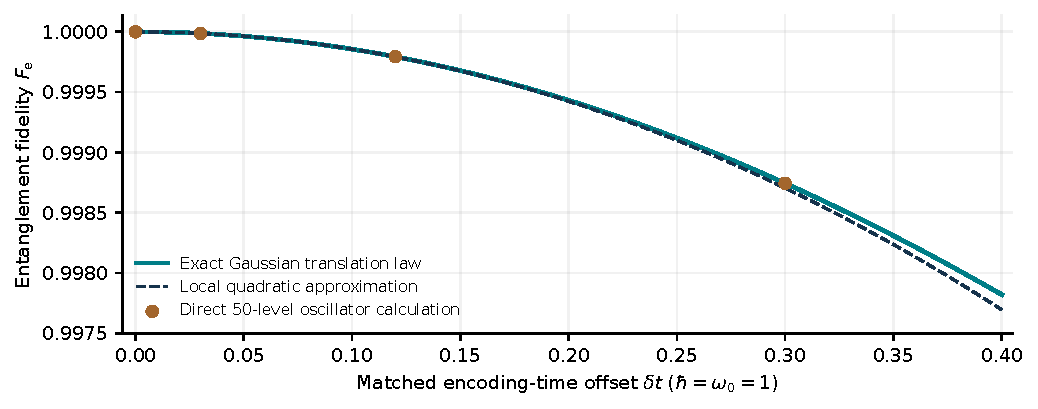
\includegraphics[width=.96\linewidth]{saddle-timing.pdf}
\caption{Timing consequences for an encoder at $t=\pi+\delta t$ and its matched coherent inverse decoder, with one noisy mode, $\hbar=\omega_0=1$, force gap 0.8 and displacement standard deviation 0.3. The solid curve is Eq.~\eqref{eq:timing-fidelity}; the dashed curve is the local quadratic approximation from Eq.~\eqref{eq:timing-expansion}; dots are independent finite-Fock calculations. Every curve and marker is keyed. The approximation need not be exact away from the turning time. No laboratory data are plotted.}
\label{fig:saddle}
\end{figure}

\section{Failure channels and information that must be retained}
\subsection{Differential translations and discarded companion information}
At the half-period, a label-dependent translation $T(\bm d_b)$ leaves $T(-\bm d_b)g$, so
\begin{equation}
 [\Lambda(\rho)]_{bc}=\rho_{bc}\langle T(-\bm d_c)g,T(-\bm d_b)g\rangle.
 \label{eq:differential}
\end{equation}
Populations can remain correct while off-diagonal coherences decay. For a real Gaussian packet with position covariance $\Sigma_g>0$ and a two-branch gap $\bm\delta=\bm d_1-\bm d_0$,
\begin{equation}
 \Gamma_{01}=e^{-\bm\delta^T\Sigma_g^{-1}\bm\delta/8},\qquad
 F_e=\frac{1+\Gamma_{01}}2.
 \label{eq:gaussian-overlap}
\end{equation}
This is an unconditional logical overlap, not a postselected projection success.

Similarly, decoding $Z$ while discarding an uncorrected branch-dependent $B$ state leaves a tag carrying logical information. For $\alpha=\beta=1/2$ and labels $(0,0),(1,1)$, the saddle heights coincide but the companion gap is one. With position standard deviation $\sigma_B=1/\sqrt2$, after known phase compensation,
\begin{equation}
 F_e^{\mathrm{omit}\,B}=\frac{1+e^{-1/4}}2=0.8894003915\ldots.
 \label{eq:omit-B}
\end{equation}
If all companion displacements are equal, that particular omission is harmless. The complete construction cannot assume this exceptional case for arbitrary design labels.

\subsection{Conjugate phase noise, erasure and matched controls}
In dimensionless auxiliary coordinates let $P(\bm\xi)=e^{\ii\bm\xi\cdot\bm Q}$ denote a transverse phase gradient, not a momentum component. At the half-period,
\begin{equation}
 E_b^\dagger T(\bm d)P(\bm\xi)E_b=e^{\ii\bm\xi\cdot\bm h_b}T(-\bm d)P(-\bm\xi).
 \label{eq:phase-gradient}
\end{equation}
For two branches and a relative path phase $\vartheta$, the remaining relative phase is $\vartheta+\bm\xi\cdot\Delta\bm h$, where $\Delta\bm h=\bm h_0-\bm h_1$. Centered joint Gaussian fluctuations give
\begin{equation}
 v=v_0+2\Delta\bm h^T\bm c+\Delta\bm h^TC_\xi\Delta\bm h,
 \quad v_0=\operatorname{Var}\vartheta,\quad\bm c=\operatorname{Cov}(\bm\xi,\vartheta).
 \label{eq:phase-variance}
\end{equation}
With mean residual phase $\overline\vartheta$, the Bell overlap is $(1+e^{-v/2}\cos\overline\vartheta)/2$. In particular, an uncorrected deterministic phase $\pi$ gives zero Bell overlap even if basis populations are correct.

For uniform state-independent transmission $\eta$, model a lost photon by an orthogonal vacuum output:
\begin{equation}
 \Lambda_\eta(\rho)=\eta\mathcal D_v(\rho)+(1-\eta)\Tr(\rho)\ket{\mathrm{vac}}\bra{\mathrm{vac}},\qquad
 F_e=\frac\eta2(1+e^{-v/2})
 \label{eq:erasure}
\end{equation}
for centered residual phase. The erasure term retains the reference marginal on an entangled input and contributes zero overlap with the original logical--reference Bell state. Correlated or state-dependent aperture loss needs a different model.

If $\bm c=0$, then $v\ge v_0$. A matched flat encoding has $\Delta\bm h=0$. If its transmission is at least the encoded transmission, \eqref{eq:erasure} gives no fidelity advantage for the saddle design in this specified noise model. This comparison does not exclude other codes or independently demonstrated beneficial correlations. Codes designed to correct broader phase-space errors require additional resources and assumptions.\cite{gkp,braunstein}


\begin{figure}[t]
\centering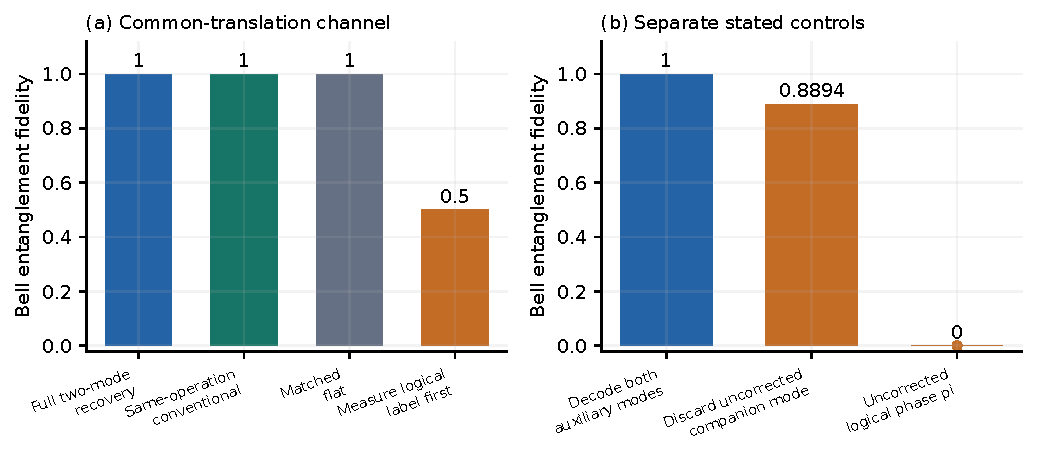
\includegraphics[width=\linewidth]{figure_4_controls.pdf}
\caption{Channel controls. (a) Under common translations, full two-mode, same-operation conventional, and matched flat recoveries all have unit Bell fidelity. Measuring the logical label first gives $1/2$ for the qubit Bell input. (b) The separate Gaussian companion-register ablation in \eqref{eq:omit-B} gives $0.8894$; an uncorrected logical phase of $\pi$ gives zero. The zero-height point marks the zero-valued bar. Values are exact or analytically evaluated; there are no statistical error bars. These are controls on different stated operations, not measured hardware comparisons.}
\label{fig:controls}
\end{figure}

\begin{figure}[t]
\centering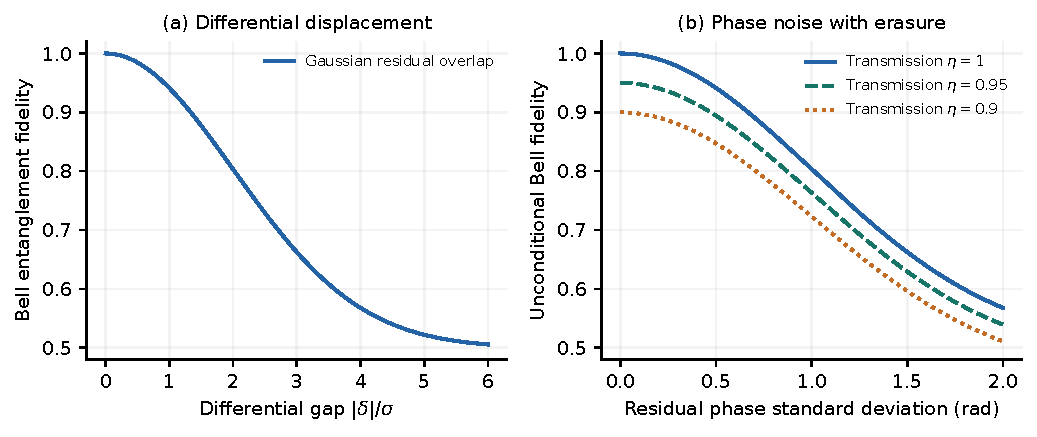
\includegraphics[width=\linewidth]{figure_5_error_limits.pdf}
\caption{Analytic limits. (a) Logical dephasing from a residual Gaussian packet gap, with other errors absent. (b) Unconditional Bell fidelity under centered Gaussian residual phase noise and uniform transmission. Solid blue, dashed green, and dotted orange curves correspond to the transmission values in the key. Every erasure is counted as failure. Curves are deterministic formulas, not fitted data; there are no uncertainty symbols or unkeyed markers.}
\label{fig:limits}
\end{figure}

\section{Candidate optical mode mapping}\label{sec:optics}
Spatial continuous-variable optics supplies a possible finite mode assignment.\cite{tasca} Let logical labels be orthogonal optical paths and the two auxiliaries be transverse coordinates within each path. The one-photon space is then $\C^d_{\mathrm{path}}\otimes L^2(\R^2)_{\mathrm{transverse}}$. The design labels $(x_b,y_b)$ index control settings, rather than two extra transverse coordinates of the same photon.

For a monochromatic scalar envelope $u_b(s,w;\ell)$ with carrier wavenumber $K=k_{\mathrm{vac}}n_{\mathrm{ref}}$, an ideal lossless paraxial model is
\begin{equation}
 \ii\partial_\ell u_b=\left[\frac{p_s^2+p_w^2}{2K}+\frac{K\Omega^2}{2}(s^2+w^2)+F_{1b}s+F_{2b}w\right]u_b.
 \label{eq:optics}
\end{equation}
Here $\Omega$ has dimensions of inverse length, and $p=-\ii\partial_q$. A parabolic-index oscillator correspondence is established optics.\cite{sauter} With $Q=\sqrt{K\Omega}\,q$, $P=p/\sqrt{K\Omega}$ and $\zeta=\Omega\ell$, the normalized force is $j_a=F_a/(\Omega\sqrt{K\Omega})$ and the half-period length is $\pi/\Omega$. Within the scalar paraxial approximation, an index prescription is
\begin{equation}
 n_b^2(s,w)=n_{\mathrm{ref}}^2-\frac{K^2\Omega^2}{k_{\mathrm{vac}}^2}(s^2+w^2)
 -\frac{2K}{k_{\mathrm{vac}}^2}(F_{1b}s+F_{2b}w).
 \label{eq:index}
\end{equation}
The prescription is restricted to a finite operating region where index squared remains positive. It does not specify a physical infinite-aperture dielectric. Fabrication, finite aperture, bandwidth, polarization, interpath coupling and control accuracy require independent evaluation.

Matching optical controls to multiples of prescribed $\kappa_b^2$ and $\tau_b^2$ is a separate calibration map. Implementing \eqref{eq:optics} would realize the stipulated Hamiltonian, not prove that a spacetime curvature field produced it. Optical propagation distance is not timelike proper time, and a null photon trajectory does not inherit the timelike Frenet frame used in Appendix~\ref{app:geometry}.

A first test would compare basis inputs, phase-sensitive superpositions and a reference-entangled input through calibrated encoding, common translations and coherent decoding. The effective logical channel should be reconstructed with erasures counted. Matched flat, same-operation conventional and no-correction controls should share the relevant transmission, timing, aperture and control accounting. The timing law \eqref{eq:timing-fidelity} gives a specific prediction to compare against controlled evolution-length errors.


The transverse coordinates in this path assignment are not the photon-number quadratures of two separate optical field modes, although both support canonical descriptions.\cite{braunstein} The continuous graph construction in Appendix~\ref{app:continuous} needs a larger logical-mode assignment and is not silently identified with this finite path implementation. A bright-beam transfer experiment can test the optical transformation, but does not by itself verify preservation of unknown quantum entanglement. In the optical normalization, the matched-time test varies the corresponding propagation length and implements the inverse of that actual transfer operation.
\section{Computational verification}
\label{sec:checks}
The accompanying package contains eight independently executable numerical scripts, including five recovery-specific checks. Their results test finite realizations and numerical consequences of the analytic statements; the proofs supply the arbitrary-input and continuum assertions.

\subsection{Exact sampled-surface register}
An exact finite model uses nine location labels $(x,y)\in\{-1,0,1\}^2$, an eleven-bin cyclic height register, and assigned height $h=x^2-y^2$ modulo eleven. It appends a basis height packet, applies the controlled shift, applies each common cyclic displacement, and decodes by the inverse shift and auxiliary trace. All $9^2\times11=891$ matrix-unit checks return the original logical operator exactly. A further 81 matrix-unit checks verify the dephasing caused by label-dependent shifts. The finite recovery's trace preservation is checked explicitly.

This cyclic model checks the geometric shear; it is not a discretization claimed to converge to an optical dielectric. Separate tests use seeded complex logical amplitudes and a complex height packet to check common-shift recovery, the differential overlap kernel, and conjugate phase action. The largest discrepancies in these dense-amplitude checks are below $1.2\times10^{-16}$ for the recorded run.

\subsection{Direct oscillator evolution and cutoff refinement}
For the dynamical test, set $\hbar=m=k=\omega=1$ and remove the common zero-point scalar. Build $Q=(a+a^\dagger)/\sqrt2$ and $P=(a-a^\dagger)/(i\sqrt2)$ in finite Fock bases. Direct spectral exponentiation of $N+JQ$ is compared with \eqref{eq:half-period}. The initial packet is $(\ket0+i\ket2)/\sqrt2$, forces are $J=-0.8,0.3,1.1$, and the common coordinate displacement is $0.4$. These signed forces test the oscillator identity; the separate two-sector test uses the positive saddle-design forces. Figure~\ref{fig:dynamics} and Table~\ref{tab:cutoff} show the cutoff dependence. Truncated canonical operators do not satisfy the infinite-dimensional commutator exactly at the boundary; refinement is therefore material to this check.

\begin{table}[ht]
\centering\small
\begin{tabular}{rrrr}\toprule
Fock dimension & Evolution discrepancy & Recovery discrepancy & $F_e$\\\midrule
20 & $7.45\times10^{-5}$ & $7.32\times10^{-5}$ & $0.9999999987542595$\\
40 & $8.07\times10^{-15}$ & $1.13\times10^{-14}$ & $0.9999999999999988$\\
60 & $6.61\times10^{-15}$ & $9.23\times10^{-15}$ & $0.9999999999999988$\\\bottomrule
\end{tabular}
\caption{Direct forced-oscillator checks. Discrepancies are maximum state-vector 2-norm differences over the three forces, not statistical uncertainties. The Bell test uses a three-level logical reference. Values are rounded directly from the fresh verification outputs; floating-point values accompany the paper.}
\label{tab:cutoff}
\end{table}



\subsection{Two-sector saddle and error-channel checks}
The two-sector test uses the nine design points, $J_0=0.1$, $\alpha=0.25$, and $\beta=0.15$ in \eqref{eq:forces}, with ground-state auxiliary packets. Direct evolution at Fock dimensions 18, 30, and 42 verifies both displacement means. Between encoder and decoder it applies common $Z,B$ translations $0.4,-0.2$, transformed back to the $S,W$ axes. At dimension 42, the maximum combined residual-state discrepancy is below $2.2\times10^{-15}$. The nine-level Bell fidelity is $0.9999999999999993$. The forward-half-period plus logical-phase decoder is checked separately and agrees to the same precision. This evaluates all 81 pairwise logical coherences through the residual-state overlaps, rather than testing only logical populations.

The phase/loss check verifies \eqref{eq:phase-gradient} using directly evolved oscillator states, \eqref{eq:phase-variance} using 16-point Gauss--Hermite quadrature in each of three Gaussian variables, and \eqref{eq:erasure} with an explicit reference-qubit times qubit-plus-vacuum output density matrix. Discrepancies are below $2.1\times10^{-15}$. Trace, positivity, and erasure-state bookkeeping are checked. These numerical results are synthetic consistency checks, not experimental fidelity measurements or an exhaustive numerical proof for all parameters.


\subsection{General criterion and timing checks}
Eighteen checks in \texttt{verify\_model.py} test the constrained action/current identities, history expansion, basis covariance, 150 sampled internal response cases, residual-state dispersion, common cyclic shifts, timing kernels, a commensurate-frequency example, uniform-circle quadrature and geometric/conservation identities. In the finite translation model, nine logical labels and an eleven-bin cyclic register give 891 common-shift matrix-unit identities. These are exact discrete checks, not a claim of continuum optical convergence.

For the timing law, direct spectral exponentiation in a 50-level Fock basis uses $H_J=N+JQ$ in normalized units, initial packet $(\ket0+\ii\ket2)/\sqrt2$, forces $-0.35$ and $0.45$, and Gaussian translation standard deviation 0.3. Fourteen-point Gauss--Hermite quadrature computes the overlap independently of \eqref{eq:timing-kernel}. Table~\ref{tab:timing} compares the results.
\begin{table}[tb]
\caption{Timing benchmark, $t=\pi+\delta t$, with all disturbances included. The formula values are deterministic analytic predictions.}
\label{tab:timing}
\begin{ruledtabular}\begin{tabular}{cccc}
$\delta t$ & Phase variance $v$ & $F_e$ from Eq.~\eqref{eq:timing-fidelity} & Comparison tolerance\\
0 & 0 & 1 & $3\times10^{-12}$\\
0.03 & 0.0000518244 & 0.9999870441 & $3\times10^{-12}$\\
0.12 & 0.0008254663 & 0.9997936760 & $3\times10^{-12}$\\
0.30 & 0.0050303343 & 0.9987439966 & $3\times10^{-12}$
\end{tabular}\end{ruledtabular}
\end{table}
The last column is the acceptance tolerance of the direct comparison, not a statistical error bar. The recorded absolute discrepancies are below $10^{-14}$ in this run. A separate oscillator check at Fock dimensions 20, 40 and 60 shows why cutoff refinement matters: a maximum half-period state discrepancy about $7.45\times10^{-5}$ at dimension 20 decreases below $10^{-13}$ at dimensions 40 and 60. Finite truncated canonical matrices do not satisfy the infinite-dimensional commutation relation at their boundary.


\begin{figure}[tb]
\centering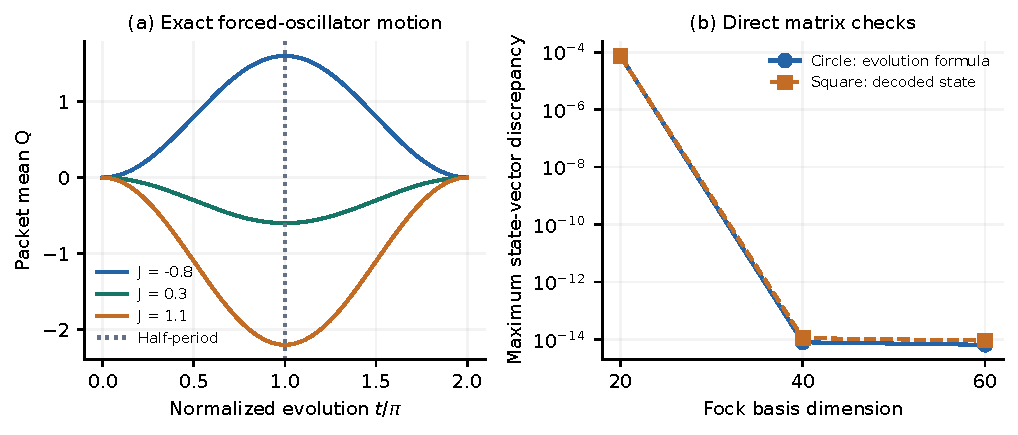
\includegraphics[width=.98\linewidth]{figure_3_dynamics.pdf}
\caption{Direct oscillator checks in normalized units. Left: exact centered-packet mean $\langle Q(t)\rangle=-J(1-\cos t)$ for each keyed force; the dotted line marks the half-period. Right: maximum state-vector discrepancies for the evolution formula (circles) and recovered states (squares) as the Fock dimension increases. Connecting lines guide the eye. The numerical values are deterministic, not sampling uncertainties.}
\label{fig:dynamics}
\end{figure}


\subsection{Full-state integration and decoder-assumption checks}
An additional script, \texttt{check\_integrated\_recovery.py}, directly propagates a complex logical state and a reference-entangled input through a controlled encoding, a four-component random-unitary mixture and coherent decoding. Partial tracing of the full density matrix is compared with the residual-state Gram channel and its fidelity-deficit identity. Phase-only residual tags verify why equality of auxiliary density matrices is insufficient without equality of their vector phases. Gaussian quadrature checks the nonzero-mean and singular-covariance case. Finally, a zero-noise oscillator comparison distinguishes a matched inverse decoder from a second forward evolution with nominal half-period phase compensation. At a nonzero timing offset the latter generally leaves logical error even though matched inverse decoding remains exact with zero noise. In the 40-level zero-noise control at $t=\pi+0.12$, with forces $-0.35,0.45$ and packet $(\ket0+\ii\ket2)/\sqrt2$, matched inversion gives unit fidelity to numerical precision, while nominal forward-phase decoding gives $F_e=0.9848610681$. This verifies the scope of the timing experiment rather than extending its noise claim.

\section{Discussion and conclusion}
The residual-state theorem states exactly which information must be retained in this controlled-noise setting. Recovery preserves an unknown logical state and its reference entanglement when the decoded auxiliary vectors, including their phases, are independent of logical label. Their pairwise separation quantifies the entanglement-fidelity deficit, and proximity to one common residual gives a sufficient diamond-norm bound. These are operational specializations of established error-correction and dilation principles.\cite{knill,kribs,ksw}

For prescribed forced oscillators, the half-period encoder produces the saddle together with its companion coordinate, parity and logical phase. The inverse operation cancels the branch-dependent encoding while common translations remain only in the auxiliaries. The general-time calculation identifies the force differences, noisy directions and turning times that determine whether a matched inverse decoder succeeds. Its quadratic timing coefficient is a controlled prediction for that experiment, not a claim covering unspecified decoder errors.

The failure cases are equally important: differential shifts can leave distinguishable residuals, discarding the companion can leak label information, phase gradients can leave relative logical phases, and erasure reduces unconditional fidelity. Matched conventional and flat controls have the same protection under the declared common noise. No intrinsic curvature advantage, arbitrary phase-space correction, photon-loss code or experimentally validated apparatus follows from this construction.

The appendices preserve the classical and geometric calculations as independently defined results. They do not establish a common microscopic theory connecting scalar localization, spinorial data, the quantum register, molecular shape and a self-consistent cosmological background. Those limits do not enter the channel proof as unproved premises. The resulting contribution is a self-contained conditional encoding and recovery construction with explicit numerical tests and a proposed optical realization.

\section*{Supplementary material}
The accompanying source archive includes the eight numerical scripts, recorded results, figure-generation code and reproduction instructions. All calculations use specified synthetic inputs. Mathematical appendices are included in this manuscript so their definitions, proofs and qualifications remain available to the reader.

\section*{Author declarations}
\subsection*{Conflict of interest}
The author declares no conflicts of interest.
\subsection*{Funding}
No external funding supported this work.
\subsection*{Author contributions}
Jason Duran Dutton: Conceptualization; methodology; formal analysis; investigation; software; validation; visualization; writing--original draft; writing--review and editing.
\section*{Data availability}
No experimental data were generated or analyzed. The accompanying source archive contains the numerical inputs, executable scripts, recorded results, scalar profiles, manuscript source and original figures. A SHA-256 manifest identifies the files. No public archival identifier has been assigned. The numerical checks test the specified implementations and finite calculations; the proofs state the general results and assumptions.

\appendix
\section{Continuous graph encoding}
\label{app:continuous}
For a continuous logical coordinate $r\in D\subseteq\mathbb R^2$ and a measurable real height function $h$, the one-auxiliary-coordinate shear acts as
\begin{equation}
 (U_h\Psi)(r,z)=\Psi(r,z-h(r)).
 \label{eq:continuousU}
\end{equation}
Integration in $z$ shows it is unitary. The encoding $(V_h\psi)(r,z)=\psi(r)g(z-h(r))$ is isometric for normalized $g$. Its inverse shear, followed by auxiliary trace, recovers the logical state under arbitrary mixtures of common height translations. The proof is the same operator factorization as in Sec.~\ref{sec:recovery}, with no parity for this directly specified geometric shear.

For a branch-dependent shift $d(r)$ the reduced density kernel is multiplied by
\begin{equation}
 \langle T(d(r'))g|T(d(r))g\rangle.
\end{equation}
Thus the coherence criterion extends over the full surface rather than only two samples. The encoding remains quantum structure introduced explicitly; it is not obtained by replacing a classical trajectory by a probability density. Lateral translations of $r$ change the logical state and are not undone by subtracting height alone. None of these statements assigns a physical four-coordinate single-photon implementation to the continuous logical register plus two dynamical auxiliaries.

\section{Constrained scalar-field representation}\label{app:scalar}
\subsection{Variables, action and real constraint}
Let $(M,g)$ be a time-oriented globally hyperbolic four-dimensional Lorentzian spacetime with signature $(+---)$. Initially the metric is prescribed. Let $\psi:M\to\C$ be a classical complex field and $\rho=|\psi|^2$. In units $c=\hbar=1$ for the classical field sections, take
\begin{equation}
 S[\psi]=\int_M\sqrt{-g}\,\dd^4x\left[\nabla_\mu\psi^*\nabla^\mu\psi-U(\rho)\right],\qquad
 \square_g\psi+U'(\rho)\psi=0,
 \label{eq:scalar-action}
\end{equation}
where $U$ is real and sufficiently differentiable. Statements about conserved integrated quantities additionally require regularity, integrability and boundary-flux conditions appropriate to the setting.

Define the dual representation and a reality involution by
\begin{equation}
 \Ph=\mathcal B\psi=\frac1{\sqrt2}\binom{\psi}{\psi^*},\qquad
 \mathcal C\binom{z_+}{z_-}=\binom{z_-^*}{z_+^*},\qquad J=\Jm.
 \label{eq:embedding}
\end{equation}
The map $\mathcal C$ is antilinear, $\mathcal C^2=\Id$, and $\mathcal C\Ph=\Ph$. Conversely every fixed vector has the form \eqref{eq:embedding}. Here $\mathcal C$ is a specified classical reality operation, not a complete definition of physical charge conjugation on a quantum field theory.

\begin{proposition}[Exact constrained dual representation]
On $\operatorname{Fix}\mathcal C$, the doublet action
\begin{equation}
 S_D[\Ph]=\int\sqrt{-g}\,\dd^4x\left[(\nabla_\mu\Ph)^\dagger\nabla^\mu\Ph-U(\Ph^\dagger\Ph)\right]
 \label{eq:doublet-action}
\end{equation}
equals \eqref{eq:scalar-action}. The scalar equation and its complex conjugate imply
\begin{equation}
 \square_g\Ph+U'(\Ph^\dagger\Ph)\Ph=0.
 \label{eq:doublet-pde}
\end{equation}
Whenever the unrestricted doublet Cauchy problem is unique in the selected regularity class, initial data satisfying $\mathcal C\Ph=\Ph$ and the corresponding condition on the normal derivative remain in that fixed subspace.
\end{proposition}
\begin{proof}
The identities $\Ph^\dagger\Ph=|\psi|^2$ and $(\nabla_\mu\Ph)^\dagger\nabla^\mu\Ph=\nabla_\mu\psi^*\nabla^\mu\psi$ follow by substitution. Since the equation has real scalar coefficients, $\mathcal C$ sends a doublet solution to another solution. The transformed and original data agree; uniqueness in the stated class therefore preserves the constraint.
\end{proof}

The factor $1/\sqrt2$ prevents double counting of the action and energy. At a spacetime point the constrained pair contains two real field components, whereas an unrestricted complex doublet contains four. Their Cauchy data have the corresponding difference in independent content. The constrained subspace is real-linear, not complex-linear: for a nonzero fixed $\Ph$, $\mathcal C(\ii\Ph)=-\ii\Ph$. Thus arbitrary complex superposition in a quantum Hilbert space is not established by imposing this classical reality constraint.

\subsection{Phase orientation and the internal orbit}
Where $\psi\ne0$, write $\psi=f e^{-\ii\theta}$ with real $f>0$. The two components of \eqref{eq:embedding} then have phase gradients $p_\mu=\nabla_\mu\theta$ and $-p_\mu$. For a future-directed unit observer $u$, their local phase rates are $\Omega_\pm(u)=\pm u^\mu\nabla_\mu\theta$. If $p$ is timelike, these gradients have opposite temporal orientations. If $p$ is null or spacelike, that timelike classification does not apply; at a field zero the phase description can fail.

On a periodic Minkowski box, an exact example is
\begin{equation}
 \psi(t)=a e^{-\ii\omega t},\qquad |a|^2=R^2,\qquad \omega^2=U'(R^2)>0,
 \qquad \Ph(t)=e^{-\ii\omega Jt}\Ph(0).
 \label{eq:orbit}
\end{equation}
Each component traces a circle in its complex plane, with opposite senses of phase evolution and a common amplitude. This orbit lies in the complex amplitude plane; it is not a spatial trajectory.

\begin{proposition}[Regular timelike orientation does not reverse continuously]
A $C^1$ timelike immersion on a connected parameter interval cannot change between the future and past timelike cones while remaining a regular timelike immersion.
\end{proposition}
\begin{proof}
In a Minkowski chart, timelikeness implies $|\dot y^0|>|\dot{\bm y}|$. The continuous quantity $\dot y^0$ cannot vanish, so its sign cannot change. The same conclusion follows from the two components of the timelike cone and a continuous time orientation on a Lorentzian manifold.
\end{proof}
Opposite phase rates in the constrained representation are distinct from reversal of the temporal orientation of a regular timelike trajectory. The representation is classical and does not specify a quantum field theory.

\subsection{Currents, energy and an optional gauge coupling}
For an unrestricted doublet with invariant potential, a constant Hermitian generator $A$ gives the Noether current
\begin{equation}
 j_A^\mu=\ii\left[\Ph^\dagger A\nabla^\mu\Ph-(\nabla^\mu\Ph)^\dagger A\Ph\right].
 \label{eq:current}
\end{equation}
On the constrained representation,
\begin{equation}
 j_{\Id}^\mu=0,\qquad
 j_J^\mu=\ii\left[\psi^*\nabla^\mu\psi-(\nabla^\mu\psi)^*\psi\right].
 \label{eq:restricted-current}
\end{equation}
The scalar phase symmetry is represented by $\Ph\mapsto e^{\ii\alpha J}\Ph$; a common doublet phase rotation is generally not a symmetry of the constrained state space. For \eqref{eq:orbit}, $j_J^0=2\omega R^2$, while the energy density is $\omega^2R^2+U(R^2)$. Opposite phase frequencies do not require a negative-energy component.

In flat spacetime the energy and stress tensor are
\begin{align}
 E&=\int_{\R^3}\left(|\partial_t\psi|^2+|\nabla\psi|^2+U\right)\dd^3x,\label{eq:energy}\\
 T_{\mu\nu}&=2\operatorname{Re}(\nabla_\mu\psi^*\nabla_\nu\psi)
 -g_{\mu\nu}\left(\nabla_\alpha\psi^*\nabla^\alpha\psi-U\right).
 \label{eq:stress}
\end{align}
For $U\ge0$ this energy is nonnegative. Conservation requires the stated boundary conditions. On curved spacetime, covariant stress conservation alone need not yield a globally conserved energy without an appropriate spacetime symmetry.\cite{wald}

A possible electromagnetic extension uses $D_\mu\psi=(\nabla_\mu+\ii eA_\mu)\psi$. Its paired form is $D_\mu\Ph=(\nabla_\mu+\ii eA_\mu J)\Ph$, so the two entries carry opposite representation weights. This is the usual scalar gauge-coupling construction;\cite{weinberg} $e$ is an assigned coupling, and the constrained pair remains one complex scalar. The gauge coupling is an input to this scalar model, not a prediction of the conjugate representation.

\begin{figure}[tb]
\centering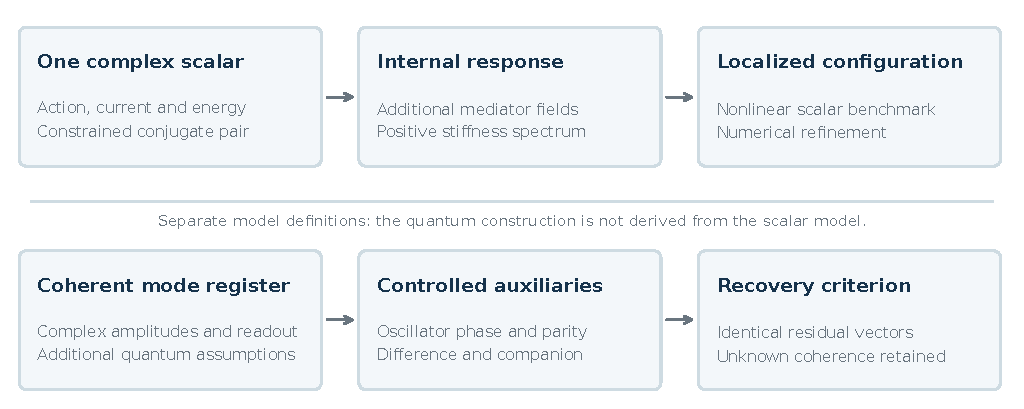
\includegraphics[width=.96\linewidth]{model-structure.pdf}
\caption{Definitions and modeling steps. The constrained classical pair contains the same independent field information as one complex scalar. Coherent logical modes and auxiliary registers are introduced with their own quantum assumptions. The arrows indicate modeling steps; the quantum register is not derived by quantizing the displayed scalar system.}
\label{fig:model}
\end{figure}

\section{Internal response, spectra and localization}\label{app:internal}
\subsection{A positive internal-field extension}
To describe internal response, introduce four real fields $I\in\R^4$ with
\begin{align}
 \mathcal L&=\nabla\psi^*\nabla\psi+\tfrac12\nabla I^T\nabla I-V(\rho,I),\\
 V&=m^2\rho+\frac\eta3\rho^3+\frac{\mu^2}{2}I^TKI-\rho\bm h^TI,
 \label{eq:potential}\\
 K&=\begin{pmatrix}1&0&0&0\\0&1&a&b\\0&a&1&0\\0&b&0&1\end{pmatrix},\qquad
 r=\sqrt{a^2+b^2}<1.
 \label{eq:K}
\end{align}
Here $m,\mu,\eta>0$ and $\bm h$ is real. The components are numbered real mediator fields. In four-dimensional mass units, $[\psi]=[I]=1$, $[\rho]=2$, $[\bm h]=1$, $[\eta]=-2$ and $[V]=4$. The sextic term is an effective classical interaction; ultraviolet completeness is not asserted.

Variation gives a reciprocal system,
\begin{equation}
 \square_g\psi+(m^2+\eta\rho^2-\bm h^TI)\psi=0,\qquad
 (\square_g+\mu^2K)I=\bm h\rho.
 \label{eq:coupled}
\end{equation}
The constrained doublet representation remains valid because the scalar coefficient is real. Four internal mediators are additional degrees of freedom in this extension; describing the underlying scalar as one field does not remove them.

\begin{proposition}[Internal spectrum and a local-response bound]
The eigenvalues of $K$ are $1,1,1-r,1+r$. A particular flat-spacetime Fourier response with no independent homogeneous mediator wave has coefficient
\begin{equation}
 \mathcal G(q)=\bm h^T(\mu^2K+q\Id)^{-1}\bm h,\qquad q=|\bm k|^2-\nu^2,\qquad G=\mathcal G(0).
 \label{eq:response}
\end{equation}
If $\delta=|q|/[\mu^2(1-r)]<1$, then
\begin{equation}
 |\mathcal G(q)-G|\le\frac{\delta}{1-\delta}G,\qquad
 \mu^2G=h_1^2+h_3^2+h_4^2+\frac{(h_2-ah_3-bh_4)^2}{1-r^2}.
 \label{eq:response-bound}
\end{equation}
\end{proposition}
\begin{proof}
One coordinate decouples; the remaining characteristic polynomial is $(1-\lambda)[(1-\lambda)^2-r^2]$. In an orthogonal eigenbasis, $\mathcal G$ is a sum of inverse denominators $\mu^2\lambda_j+q$ with nonnegative squared coupling weights. Each term changes from its zero-frequency value by relative magnitude at most $\delta/(1-\delta)$. Summation gives the bound. Eliminating coordinates 3 and 4 gives the displayed Schur-complement formula.
\end{proof}
The estimate controls a multiplier in its specified band. It is not a nonlinear continuation theorem for field solutions. Initial data generally contain homogeneous mediator waves, and a retarded prescription has to be stated rather than inferred from the inverse matrix.

The leading local substitution $\bm h^TI\simeq G\rho$ gives
\begin{equation}
 U_{\mathrm{loc}}(\rho)=m^2\rho-\frac G2\rho^2+\frac\eta3\rho^3.
 \label{eq:local-potential}
\end{equation}
Completing the square in the full potential gives
\begin{equation}
 V=\frac{\mu^2}{2}\left(I-\mu^{-2}K^{-1}\bm h\rho\right)^TK
 \left(I-\mu^{-2}K^{-1}\bm h\rho\right)+U_{\mathrm{loc}}(\rho).
 \label{eq:square}
\end{equation}
The minimum of $U_{\mathrm{loc}}(\rho)/\rho$ on $\rho\ge0$ is $m^2-3G^2/(16\eta)$. Thus $m^2>3G^2/(16\eta)$ supplies a nonnegative potential with zero vacuum. This lower bound and conservation of energy are distinct properties; neither by itself proves nonlinear stability of every solution.

\subsection{A well-defined linear spectral problem}
For a closed compact Riemannian spatial slice $\Sigma$, define
\begin{equation}
 A=-\Delta_\Sigma\otimes\Id_4+\mu^2K+W(x)\Id_4,
 \quad D(A)=H^2(\Sigma;\C^4),\quad W\in C^\infty(\Sigma;\R),\quad W\ge0.
 \label{eq:spatial-spectrum}
\end{equation}
This is a positive self-adjoint elliptic operator with compact resolvent.\cite{reed,rosenberg} Indeed, $-\Delta_\Sigma$ has those domain properties, and the real smooth multiplication and finite internal matrix are bounded symmetric perturbations. Its quadratic form has lower bound $\mu^2(1-r)$. Standard compact Sobolev embedding gives compact resolvent. If $W=W_0$ is constant, the eigenvalues are exactly
\begin{equation}
 \lambda_n(-\Delta_\Sigma)+\mu^2\lambda_j(K)+W_0.
 \label{eq:separated-spectrum}
\end{equation}
This supplies an orthonormal mode expansion for a specified spatial problem. The Lorentzian wave operator on all spacetime is not being treated as that positive elliptic operator. On noncompact space, discrete spectrum requires additional hypotheses.

For $\ddot q+Aq=0$, the complexified variable $z=(A^{1/2}q+\ii\dot q)/\sqrt2$ satisfies $\ii\dot z=A^{1/2}z$ on the natural energy domain. This gives a linear amplitude description of a classical oscillator system. Interpreting its norm as a quantum probability still requires quantum state and measurement assumptions. The eigenvalues describe this specified classical linear problem.

\subsection{The nonlinear profile and a reproducible benchmark}
In the local flat-space scalar model, set $\psi=f(\bm x)e^{-\ii\omega t}$ with real decaying $f$. Then
\begin{equation}
 \left[-\Delta+m^2-Gf^2+\eta f^4\right]f=\omega^2f.
 \label{eq:nonlinear-spectrum}
\end{equation}
The operator depends on its unknown profile; this is not the fixed linear spectrum \eqref{eq:spatial-spectrum}. The familiar attractive--sextic scalar theory provides the localization benchmark.\cite{coleman,nugaev} The standard frequency condition suggested by $\min_{\rho>0}U_{\mathrm{loc}}/\rho<\omega^2<U_{\mathrm{loc}}'(0)$ is
\begin{equation}
 m^2-\frac{3G^2}{16\eta}<\omega^2<m^2.
 \label{eq:frequency-window}
\end{equation}
This condition is not a proof of stability for the mediator system.

For $m=\eta=1$, $G=2$, $\omega=0.8$, solve
\begin{equation}
 f''+\frac2r f'=(1-\omega^2)f-2f^3+f^5,\qquad f'(0)=0,\qquad f(R)=0.
 \label{eq:radial}
\end{equation}
The packaged scalar solver uses a regular origin stencil, damped Newton iteration and a tridiagonal linear solve. With $K_f=\int|\nabla f|^2$, $I_f=\int f^2$ and $V_f=\int U_{\mathrm{loc}}(f^2)$, the stationary scaling identity is
\begin{equation}
 K_f+3V_f-3\omega^2I_f=0.
 \label{eq:virial}
\end{equation}
Table~\ref{tab:radial} records the regenerated calculation. Its relative virial discrepancy is the absolute left side of \eqref{eq:virial} divided by $K_f+3V_f+3\omega^2I_f$.
\begin{table}[tb]
\caption{Dimensionless local radial benchmark, $R=30$. Residual is the maximum discrete equation residual. All entries are deterministic numerical results for the specified scalar model.}
\label{tab:radial}
\begin{ruledtabular}\begin{tabular}{ccccc}
Grid spacing & $f(0)$ & Energy & Residual & Relative virial discrepancy\\
0.1 & 1.286969 & 177.15166 & $1.26\times10^{-12}$ & $1.09\times10^{-4}$\\
0.05 & 1.287055 & 177.23919 & $3.10\times10^{-13}$ & $2.73\times10^{-5}$\\
0.025 & 1.287076 & 177.26105 & $1.58\times10^{-12}$ & $6.82\times10^{-6}$\\
\end{tabular}\end{ruledtabular}
\end{table}
The finest-grid charge is $Q_J=190.39440$ and $E/Q_J=0.93102$. Increasing $R$ to 40 at that spacing changes the quoted energy by less than $10^{-9}$. The virial discrepancy decreases by approximately four on halving the spacing. Domain agreement and a small equation residual do not establish continuum orbital stability or continuation to the full finite-range or gravitational model.

\begin{proposition}[A complementary localization obstruction]
For $U(\rho)=m^2\rho+g\rho^2/2$, $g>0$, there is no nonzero regular decaying time-harmonic $H^1(\R^3)$ profile for which the following integrations and vanishing-boundary identities hold.
\end{proposition}
\begin{proof}
The equation is $-\Delta f+(m^2-\omega^2)f+gf^3=0$. Put $A_f=\int|\nabla f|^2$, $B_f=(m^2-\omega^2)\int f^2$ and $C_f=g\int f^4$. Multiplication by $f$ and stationary spatial scaling give $A_f+B_f+C_f=0$ and $A_f/2+3B_f/2+3C_f/4=0$. Eliminating $B_f$ yields $A_f+3C_f/4=0$, forcing $f=0$.
\end{proof}
An internal phase circle is therefore insufficient to bind an object. The potential and field equations supply substantive dynamical information.

\begin{figure}[tb]
\centering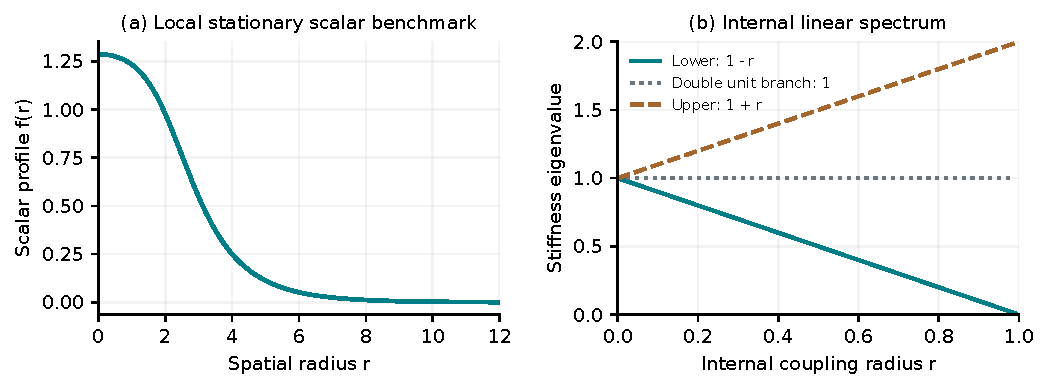
\includegraphics[width=.96\linewidth]{localization-spectrum.pdf}
\caption{Left: the regenerated radial profile of the local scalar benchmark at $\omega=0.8$, grid spacing 0.025 and $R=30$. Right: stiffness branches $1-r$, $1$ and $1+r$, with the second unit branch coincident. The profile and stiffness eigenvalues belong to distinct specified problems; neither is an experimental measurement.}
\label{fig:localization}
\end{figure}

\section{Coherent histories and specified detector response}\label{app:histories}
\subsection{The amplitude data that interference requires}
Let a finite layered set of spatial sites have a fixed number $d$ of modes per layer. An edge is allowed only when its spatial separation is at most $v\Delta t$. Choose unitary matrices $U_j$ whose nonzero entries obey the allowed edges, and a normalized input $c\in\C^d$. This is a specified coherent finite-history model, consistent with standard quantum walks.\cite{aharonov,kempe} Existence of a unitary with a selected sparsity pattern is an assumption, not a property of every causal graph.

For a history $h=(r_0,\ldots,r_n)$ put
\begin{equation}
 \mathcal A(h)=c_{r_0}\prod_{j=1}^n(U_j)_{r_jr_{j-1}},\qquad
 \Psi_n(r)=\sum_{h:r_n=r}\mathcal A(h).
 \label{eq:histories}
\end{equation}
Expanding a finite matrix product proves $\Psi_n=U_n\cdots U_1c$ and $\|\Psi_n\|=1$. A declared Born readout $p_n(r)=|\Psi_n(r)|^2$ contains the cross terms between histories with a common output. Replacing the amplitudes by positive history weights before summation removes that information.

For example, take $H=2^{-1/2}\bigl(\begin{smallmatrix}1&1\\1&-1\end{smallmatrix}\bigr)$ and $D_\alpha=\operatorname{diag}(1,e^{\ii\alpha})$. Then
\begin{equation}
 HD_\alpha H\binom10=\frac12\binom{1+e^{\ii\alpha}}{1-e^{\ii\alpha}},\qquad
 p_\pm=\frac{1\pm\cos\alpha}{2}.
 \label{eq:interference}
\end{equation}
Two sites at separation $\ell$ and layer spacing $\Delta t>\ell/v$ allow all of these transitions within the chosen causal bound. With normalized detector tags $d_0,d_1$, tracing the tag gives
\begin{equation}
 p_\pm=\frac{1\pm\operatorname{Re}(e^{\ii\alpha}\langle d_0,d_1\rangle)}2,\qquad
 \mathcal V=|\langle d_0,d_1\rangle|.
 \label{eq:visibility}
\end{equation}
This is the established which-path coherence mechanism.\cite{englert} It is also the structure that reappears in the recovery theorem in the main text.

The transformation $c\mapsto R_0c$, $U_j\mapsto R_jU_jR_{j-1}^\dagger$, with diagonal unitary $R_j$, changes $\Psi_n$ to $R_n\Psi_n$ and leaves output probabilities unchanged. Intermediate basis phases cancel in each history. Relative phase at a common output, rather than an arbitrary basis convention, controls interference.

\subsection{A detector map is additional structure}
For a classical observation specification $\mathcal D$ with channel sensitivity $\ell$, reference $\beta$ and nonnegative sampling window $W$, one possible response is
\begin{equation}
 \mathcal R_{\mathcal D}[\Ph,g]=\int W(x)\,|\ell^\dagger(x)\Ph(x)+\beta(x)|^2\,\dd\mu_g(x).
 \label{eq:detector}
\end{equation}
Its interpretation depends on a calibrated detector interaction. Quantum detector theory instead uses a specified quantum field state and detector coupling, often through a two-point correlation function.\cite{unruh,louko} A localized classical stress--energy concentration, an optical intensity and a quantum detection event are distinct objects. Neither the conjugate-pair construction nor an observer's trajectory alone selects a universal measurement law.

\section{Prescribed histories and invariant geometry}
\label{app:geometry}
For a unit timelike tangent $T$ in a Minkowski $1+2$ subspace with metric $\eta=\operatorname{diag}(1,-1,-1)$, take constant $\kappa>0$ and real $\tau$. The Frenet equations are
\begin{equation}
 T'=\kappa N,\quad N'=\kappa T+\tau B,\quad B'=-\tau N,\qquad
 F'=FA,\quad A=\begin{pmatrix}0&\kappa&0\\\kappa&0&-\tau\\0&\tau&0\end{pmatrix}.
 \label{eq:frenet}
\end{equation}
Since $A^T\eta+\eta A=0$, an initial Lorentz-orthonormal frame remains so under $F(s)=F(0)e^{sA}$. Integrating $T(s)$ gives a regular timelike history with the specified invariants. This is a kinematic existence statement. It does not solve freely coupled geometry--field equations or identify a timelike history with a null photon ray.

More generally, if a smooth vector field $X$ generates a unique local flow and a regular constraint submanifold is to be invariant, the necessary tangency condition is $X(z)\in T_z\Sigma$ for every $z\in\Sigma$. Under the usual smooth embedded-submanifold hypotheses, the restricted flow and uniqueness make this condition locally sufficient. Naming a locus of fixed invariants does not prove tangency, attraction or Lyapunov stability. A retraction to that locus also need not commute with the dynamical operator.

\section{Limits of positive trajectory reconstruction}
\label{app:reconstruction}
\subsection{An exact causal-graph reduction}
Let $X$ be a compact metric space, $Z=[0,T]\times X$, and
\begin{equation}
 D_a((t,x),(s,y))=a|t-s|+d_X(x,y),\qquad a>0.
\end{equation}
Let $\mathcal C_v$ be the spatial paths with Lipschitz constant at most $v$. Let $\mathcal G_{N,v}$ contain all probability measures supported on a union of at most $N$ such spacetime graphs, without prescribing their temporal marginals. Let $\mathcal E_{N,v}$ be the smaller class of constant-weight mixtures of their coordinate-time occupations
\begin{equation}
 P_\gamma(f)=\frac1T\int_0^T f(t,\gamma(t))\dd t.
\end{equation}
For a spatial probability $\sigma$, define its standard $N$-point quantization error\cite{kloeckner}
\begin{equation}
 e_N(\sigma)=\inf_{x_1,\ldots,x_N}\int_X\min_i d_X(x,x_i)\,\sigma(\dd x).
\end{equation}
\begin{theorem}[Static-target identity]
For $\nu=(\dd t/T)\otimes\sigma$ and $a\ge v$,
\begin{equation}
 \inf_{\mu\in\mathcal G_{N,v}}W_{1,a}(\nu,\mu)
 =\inf_{\mu\in\mathcal E_{N,v}}W_{1,a}(\nu,\mu)=e_N(\sigma).
 \label{eq:quantization}
\end{equation}
\end{theorem}
\begin{proof}
For a target point $(t,x)$ and any point $(s,\gamma_i(s))$ on a supporting graph,
\begin{equation}
 a|t-s|+d_X(x,\gamma_i(s))\ge d_X(x,\gamma_i(t))+(a-v)|t-s|\ge d_X(x,\gamma_i(t)).
\end{equation}
Thus any coupling to the graph union costs at least the target average of $\min_i d_X(x,\gamma_i(t))$, which is at least $e_N(\sigma)$ at each time. Compactness of $X$ gives minimizing spatial centers. Choose measurable nearest-center cells and their $\sigma$-weights, keep each path stationary at its center, and send each cell to that center without changing time. This coupling has cost $e_N(\sigma)$ and belongs to the smaller class.
\end{proof}
For a uniform probability on a circle of circumference one, equipped with geodesic distance, $e_N=1/(4N)$. One proof uses the bound $\sigma\{\min_i d(x,x_i)\le r\}\le2Nr$ for $0\le r\le1/(2N)$, integrates its complement, and then uses equally spaced centers to attain the value. Hence a single positive causal graph has a strictly positive joint-spacetime error for this diffuse target, even though a long spatial orbit can visit all positions after time is discarded.

The cost condition is material. For $0<a<v$ and $T\ge2/v$, the path $\gamma(s)=vs\pmod1$ supports a measure with
\begin{equation}
 W_{1,a}(\nu,\mu)\le\frac a{4v}+\frac{2a}{v^2T}.
 \label{eq:cheap-time}
\end{equation}
To obtain it, send $(t,x)$ to a closest visit time $s$ with $vs=x\pmod1$. Away from the two boundary strips of total length $2/v$, the average nearest-visit offset is $1/(4v)$; in a boundary strip a visit can be chosen within $1/v$. For sufficiently large finite $T$, the upper bound is below $1/4$. This measure need not have uniform temporal marginal, so the example concerns $\mathcal G_{1,v}$, not necessarily $\mathcal E_{1,v}$.

\subsection{Ensembles, currents and spin data}
On a flat torus, a probability $\eta$ on bounded-speed paths gives positive occupation $\rho_\eta$ and flux $j_\eta$ by averaging $P_\gamma$ and $\dot\gamma P_\gamma$. The chain rule gives the distributional continuity equation in the open cylinder and $|j_\eta|\le v\rho_\eta$. This belongs to the setting of established superposition principles for currents and continuity equations.\cite{stepanov,miller} It is not a coherent amplitude sum. Uniform stationary paths and uniform mixtures of opposite constant velocities can have the same one-time density and zero mean flux, while their two-time correlations differ. Those first moments do not determine a unique underlying history law.

There is also an algebraic spin obstruction. Suppose tensorial trajectory data are unchanged by the central element $-1\in\operatorname{Spin}^+(1,3)$, while the target spinor representation changes sign. Every equivariant reconstruction $F$ then obeys $F(D)=F((-1)D)=-F(D)$ and is zero. A lifted state space or independent spinorial variables can change that conclusion; scalar occupation and tensorial current alone do not provide them.\cite{schubert}

\section{Conditional helix and cosmological mappings}
\label{app:mappings}
\subsection{Helical shape and local invariants}
For the ideal spatial helix $X(u)=(R\cos u,R\sin u,bu)$, with $b=P/(2\pi)$ and positive radius and pitch,
\begin{equation}
 \kappa=\frac R{R^2+b^2},\qquad \tau_g=\frac b{R^2+b^2},\qquad
 \frac\kappa{\tau_g}=\frac{2\pi R}P.
 \label{eq:helix}
\end{equation}
These are standard geometric invariants.\cite{kamien} They provide a conditional parameterization of helical shape. The parameter $u$ is spatial, not physical time. An embedding $X(t,u)$ instead gives a material-point worldline by fixing $u$.

One conditional internal coupling is $a=\alpha_g\kappa^2$, $b=\beta_g\tau_g^2$, with $[\alpha_g]=[\beta_g]=\mathrm{length}^2$ and $\sqrt{\alpha_g^2\kappa^4+\beta_g^2\tau_g^4}<1$ to retain the positive matrix \eqref{eq:K}. This is a prescribed coupling, not a fitted or experimentally validated constitutive relation. Independent structures, uncertainties, response calibration and held-out comparisons against standard molecular or elastic models would be needed.\cite{drew} For example, $R=10.5$ \AA\ and $P=34$ \AA\ give $\kappa/\tau_g=21\pi/34\simeq1.9404$; this numerical ratio depends on the chosen dimensions and is not a universal constant.

\subsection{Expansion, current and energy}
On prescribed flat Friedmann--Lema\^itre--Robertson--Walker spacetime $\dd s^2=\dd t^2-a(t)^2\dd\bm x^2$, a homogeneous field satisfies
\begin{equation}
 \ddot\psi+3H\dot\psi+U'(|\psi|^2)\psi=0,\qquad H=\dot a/a.
 \label{eq:cosmo-pde}
\end{equation}
For $\psi=f(t)e^{-\ii\theta(t)}$, current conservation gives $a^3f^2\dot\theta=\mathrm{constant}$ and $j^0\propto a^{-3}$. It does not imply that $f$ itself always scales as $a^{-3}$. The scalar stress instead satisfies
\begin{equation}
 \epsilon=|\dot\psi|^2+U,\quad p=|\dot\psi|^2-U,\qquad
 \dot\epsilon+3H(\epsilon+p)=0.
 \label{eq:cosmo-energy}
\end{equation}
These are ordinary covariant conservation relations.\cite{wald,turner}

For $U=m^2|\psi|^2$, the prescribed background $a=(t/t_0)^{2/3}$ admits
\begin{equation}
 \psi(t)=\frac{t_0}t e^{-\ii mt}a_0,\quad t>0,\qquad
 j^0=\frac{2m|a_0|^2t_0^2}{t^2},\quad
 \epsilon=|a_0|^2t_0^2\left(\frac{2m^2}{t^2}+\frac1{t^4}\right),\quad
 p=\frac{|a_0|^2t_0^2}{t^4}.
 \label{eq:cosmo-example}
\end{equation}
Direct differentiation verifies the field equation and continuity relation. The energy contains both $a^{-3}$ and $a^{-6}$ pieces. This stress does not by itself exactly source the assigned $a\propto t^{2/3}$ background: its energy has an extra $t^{-4}$ dependence not present in $H^2$. A self-consistent gravitational model must also satisfy the appropriate Einstein constraints, for example $H^2=8\pi G_N\epsilon/3$ and $\dot H=-4\pi G_N(\epsilon+p)$ with all retained fields included. The example verifies conservation on a prescribed background; it is not a self-consistent solution of the coupled gravitational system.


\section{Reproduction and audit trail}
With a Python environment satisfying the dependencies in \texttt{requirements.txt}, run
\begin{verbatim}
python run_checks.py
python make_recovery_figures.py
python make_field_figures.py
python make_highlight.py
\end{verbatim}
The verification runner executes all eight scripts in \texttt{numerical/}, including the radial grid and domain checks. The standard-library recovery checks and NumPy calculations retain their declared synthetic inputs; figures are generated with Matplotlib. Compile \texttt{Conjugate\_Phase\_Geometry\_AIP\_Advances.tex} with pdfLaTeX at least twice to settle citations and references. A build script and source-to-result integration map accompany the package. No remote account or hardware backend is needed.
\begin{thebibliography}{99}
\bibitem{feynman}R. P. Feynman, ``Space-time approach to non-relativistic quantum mechanics,'' Rev. Mod. Phys. \textbf{20}, 367--387 (1948), \href{https://doi.org/10.1103/RevModPhys.20.367}{doi:10.1103/RevModPhys.20.367}.
\bibitem{aharonov}Y. Aharonov, L. Davidovich, and N. Zagury, ``Quantum random walks,'' Phys. Rev. A \textbf{48}, 1687--1690 (1993), \href{https://doi.org/10.1103/PhysRevA.48.1687}{doi:10.1103/PhysRevA.48.1687}.
\bibitem{kempe}J. Kempe, ``Quantum random walks: An introductory overview,'' Contemp. Phys. \textbf{44}, 307--327 (2003), \href{https://doi.org/10.1080/00107151031000110776}{doi:10.1080/00107151031000110776}.
\bibitem{schubert}C. Schubert, ``Perturbative quantum field theory in the string-inspired formalism,'' Phys. Rep. \textbf{355}, 73--234 (2001), \href{https://doi.org/10.1016/S0370-1573(01)00013-8}{doi:10.1016/S0370-1573(01)00013-8}.
\bibitem{coleman}S. Coleman, ``Q-balls,'' Nucl. Phys. B \textbf{262}, 263--283 (1985), \href{https://doi.org/10.1016/0550-3213(85)90286-X}{doi:10.1016/0550-3213(85)90286-X}.
\bibitem{nugaev}E. Nugaev and A. Shkerin, ``Review of non-topological solitons in theories with U(1)-symmetry,'' \href{https://arxiv.org/abs/1905.05146}{arXiv:1905.05146} (2019).
\bibitem{knill}E. Knill and R. Laflamme, ``Theory of quantum error-correcting codes,'' Phys. Rev. A \textbf{55}, 900--911 (1997), \href{https://doi.org/10.1103/PhysRevA.55.900}{doi:10.1103/PhysRevA.55.900}.
\bibitem{kribs}D. Kribs, R. Laflamme, and D. Poulin, ``Unified and generalized approach to quantum error correction,'' Phys. Rev. Lett. \textbf{94}, 180501 (2005), \href{https://doi.org/10.1103/PhysRevLett.94.180501}{doi:10.1103/PhysRevLett.94.180501}.
\bibitem{wald}R. M. Wald, \emph{General Relativity} (University of Chicago Press, Chicago, 1984).
\bibitem{weinberg}S. Weinberg, \emph{The Quantum Theory of Fields}, Vol. I (Cambridge University Press, Cambridge, 1995).
\bibitem{reed}M. Reed and B. Simon, \emph{Methods of Modern Mathematical Physics}, Vol. I: \emph{Functional Analysis}, revised and enlarged ed. (Academic Press, New York, 1980).
\bibitem{rosenberg}S. Rosenberg, \emph{The Laplacian on a Riemannian Manifold} (Cambridge University Press, Cambridge, 1997).
\bibitem{englert}B.-G. Englert, ``Fringe visibility and which-way information: An inequality,'' Phys. Rev. Lett. \textbf{77}, 2154--2157 (1996), \href{https://doi.org/10.1103/PhysRevLett.77.2154}{doi:10.1103/PhysRevLett.77.2154}.
\bibitem{unruh}W. G. Unruh, ``Notes on black-hole evaporation,'' Phys. Rev. D \textbf{14}, 870--892 (1976), \href{https://doi.org/10.1103/PhysRevD.14.870}{doi:10.1103/PhysRevD.14.870}.
\bibitem{louko}J. Louko and A. Satz, ``How often does the Unruh--DeWitt detector click? Regularisation by a spatial profile,'' Class. Quantum Grav. \textbf{23}, 6321--6344 (2006), \href{https://arxiv.org/abs/gr-qc/0606067}{arXiv:gr-qc/0606067}.
\bibitem{docarmo}M. P. do Carmo, \emph{Riemannian Geometry} (Birkh\"auser, Boston, 1992).
\bibitem{nielsen}M. A. Nielsen, ``The entanglement fidelity and quantum error correction,'' \href{https://arxiv.org/abs/quant-ph/9606012}{arXiv:quant-ph/9606012} (1996).
\bibitem{ksw}D. Kretschmann, D. Schlingemann, and R. F. Werner, ``The information-disturbance tradeoff and the continuity of Stinespring's representation,'' IEEE Trans. Inf. Theory \textbf{54}, 1708--1717 (2008), \href{https://doi.org/10.1109/TIT.2008.917696}{doi:10.1109/TIT.2008.917696}.
\bibitem{gkp}D. Gottesman, A. Kitaev, and J. Preskill, ``Encoding a qubit in an oscillator,'' Phys. Rev. A \textbf{64}, 012310 (2001), \href{https://doi.org/10.1103/PhysRevA.64.012310}{doi:10.1103/PhysRevA.64.012310}.
\bibitem{braunstein}S. L. Braunstein and P. van Loock, ``Quantum information with continuous variables,'' Rev. Mod. Phys. \textbf{77}, 513--577 (2005), \href{https://doi.org/10.1103/RevModPhys.77.513}{doi:10.1103/RevModPhys.77.513}.
\bibitem{tasca}D. S. Tasca, R. M. Gomes, F. Toscano, P. H. Souto Ribeiro, and S. P. Walborn, ``Continuous-variable quantum computation with spatial degrees of freedom of photons,'' Phys. Rev. A \textbf{83}, 052325 (2011), \href{https://doi.org/10.1103/PhysRevA.83.052325}{doi:10.1103/PhysRevA.83.052325}.
\bibitem{sauter}E. G. Sauter and A. K. Ghatak, ``The harmonic oscillator problem and the parabolic index optical waveguide: II. Quantum mechanical and wave optical analyses,'' Eur. J. Phys. \textbf{10}, 144 (1989), \href{https://doi.org/10.1088/0143-0807/10/2/013}{doi:10.1088/0143-0807/10/2/013}.
\bibitem{kloeckner}B. Kloeckner, ``Approximation by finitely supported measures,'' ESAIM Control Optim. Calc. Var. \textbf{18}, 343--359 (2012), \href{https://doi.org/10.1051/cocv/2010100}{doi:10.1051/cocv/2010100}.
\bibitem{stepanov}E. Stepanov and D. Trevisan, ``Three superposition principles: Currents, continuity equations and curves of measures,'' J. Funct. Anal. \textbf{272}, 1044--1103 (2017), \href{https://doi.org/10.1016/j.jfa.2016.10.025}{doi:10.1016/j.jfa.2016.10.025}.
\bibitem{miller}T. Miller, ``Causal evolution of probability measures and continuity equation,'' Adv. Theor. Math. Phys. \textbf{28}, 743--804 (2024), \href{https://doi.org/10.4310/ATMP.241028222555}{doi:10.4310/ATMP.241028222555}.
\bibitem{kamien}R. D. Kamien, ``The geometry of soft materials: A primer,'' Rev. Mod. Phys. \textbf{74}, 953--971 (2002), \href{https://doi.org/10.1103/RevModPhys.74.953}{doi:10.1103/RevModPhys.74.953}.
\bibitem{drew}H. R. Drew et al., ``Structure of a B-DNA dodecamer: Conformation and dynamics,'' Proc. Natl. Acad. Sci. U.S.A. \textbf{78}, 2179--2183 (1981), \href{https://doi.org/10.1073/pnas.78.4.2179}{doi:10.1073/pnas.78.4.2179}.
\bibitem{turner}M. S. Turner, ``Coherent scalar-field oscillations in an expanding universe,'' Phys. Rev. D \textbf{28}, 1243--1247 (1983), \href{https://doi.org/10.1103/PhysRevD.28.1243}{doi:10.1103/PhysRevD.28.1243}.
\end{thebibliography}
\end{document}

